\chapter{Proposed software} % Last updated: 4-2-2016
\label{ch:software}
Time can be saved by using already written and validated software. Because of the available software from both TU Delft and \ac{JPL} and the evaluation speed it was decide to use C++ as the main programming language. Many of the software packages that are used at \ac{JPL} fall under the \ac{ITAR}. This means that the software cannot be used directly by foreign nationals, however some of the tools that are used in those software packages are commercially available. The \ac{JPL} software can nonetheless still be used as a verification tool for the software that will be written during the course of this thesis project. In that case, a \ac{JPL} employee will simulate the trajectory with the same conditions as the written software and the results can be compared to each other. For the optimisation, there is software available that can be integrated into the newly written software. In \Cref{sec:ex_soft} the different existing software packages that will be used are described and any changes that will have to be made to the software. \Cref{sec:develop_soft} describes the different aspects of the simulation program that will have to be developed during the thesis work.

\section{Existing software packages}
\label{sec:ex_soft}
As was discussed in \Cref{subsec:varmbhmeth} there is already software available for the local optimisation of the \ac{MBH} method. As a matter of fact, \ac{MBH} itself is already an option within the \ac{PaGMO} package \cite{izzo2012pygmo,boudestijn2014}. However, should \ac{PaGMO} not be available or should \ac{MBH} have to be modified, it is still usefull to have a seperate version of the local optimisation software available. During the ascent, Mars-\ac{GRAM} 2005 (originally developed in the '90s) will be used to simulate the Martian atmospheric conditions.  An overview of the software packages is provided in \Cref{tab:exissoft}.

%To determine the influence of perturbations and shadowing by the Sun, information on the relative position of the Sun with respect to Mars is required as well \cite{gebbett2014multi}. This information (Ephemeris) is provided by \ac{SPICE} (created by the \ac{NAIF} in the '80s \footnote{\label{foot:spice}NASA website: \url{https://naif.jpl.nasa.gov/naif/spicehistory.html} [Accessed 14 December 2015]}).

\begin{table}[!ht]
\begin{center}
\caption{Required existing software}
\label{tab:exissoft}
\begin{tabular}{|l|l|p{3cm}|l|p{3cm}|l|}
\hline 
\textbf{Subject} &	\textbf{Software} & \textbf{Developer} & \textbf{Year} & \textbf{C++ source code/compatible} & \textbf{Provided by} \\ \hline \hline
Optimisation & \ac{PaGMO} & \ac{ESA} Advanced Concept Team \cite{izzo2012pygmo} & 2012 & Yes & \ac{ESA} \tablefootnote{For more information on \ac{PaGMO} please see the ESA website: \url{http://esa.github.io/pagmo/} [Accessed 4 February 2016]} \\ \hline
Optimisation & \ac{SNOPT} & Gill et al. \cite{gill2002snopt} & 2002 & Yes  & TU Delft and \ac{JPL} \tablefootnote{\ac{SNOPT} is also available through\ac{PaGMO} \cite{izzo2012pygmo}} \\ \hline
Atmosphere & Mars-\ac{GRAM} 2005 & Justus \cite{justus1990mars} & 2005 & Yes & TU Delft and \ac{JPL} \\ \hline
Simulation & Tudat & Doornbos et al. \tablefootnote{Development started in 2009. For more information please see \url{http://tudat.tudelft.nl/} [Accessed 4 February 2016] This website is only accessible through the TU Delft network}  & 2009 & Yes & TU Delft \\ \hline
\end{tabular}
\end{center}
\end{table}

%Both \ac{PaGMO} and \ac{SNOPT} are available through Tudat which can be provided by the TU Delft. However, at this point it is assumed that the simulation program software will mostly be based on \ac{JPL} software.\\


In \Cref{ch:optimisation} it was already mentioned that \ac{SNOPT} will be used as the local optimisation tool for \ac{MBH}. This means that if the pre-set \ac{PaGMO} version of \ac{MBH} is used, \ac{SNOPT} will have to be incorporated into it. However, should \ac{PaGMO} not be available after all, then \ac{SNOPT} will simply be integrated into the self developed \ac{MBH} software. It is not expected that the \ac{SNOPT} software itself will require any adjustments. Also, Mars-\ac{GRAM} 2005 will solely be used for its outputs, which means that its can be run separately from the optimiser and also will not need to be changed. It could be that more changes are required when actually using the software, but these are the (possible) required changes envisioned at this time.


%Warrens Q-law (possible) changes:
%
%Integrator (used for MEE Adams-Moulton multi-step, can change to RK4 or RKF or TSI)
%Earth --> Mars
%Penalty function
%More Matlab?

\section{Development of new software}
\label{sec:develop_soft}
The final thesis topic is similar to the Earth ascent problem studied by Pagano \cite{pagano2010thesis}. Unfortunately, it is not similar enough, which means that new software will have to be developed for this thesis problem. All the tools that will have to be developed will be written in C++ and will have to be combined in the end, together with the existing software, to form the final simulation software. There are several aspects of the simulation program that will have to be written. These include: ascent dynamic equations, linear interpolation, the different integration methods, and might also include \ac{MBH}. Preferably these will all be written as separate tools and such that they are flexible enough to also be applied to other problems. The top-level architecture of the program as it is currently envisioned can now be set up, and is visualised in \Cref{fig:general_soft_architecture}.

\begin{figure}[!ht]
\centering
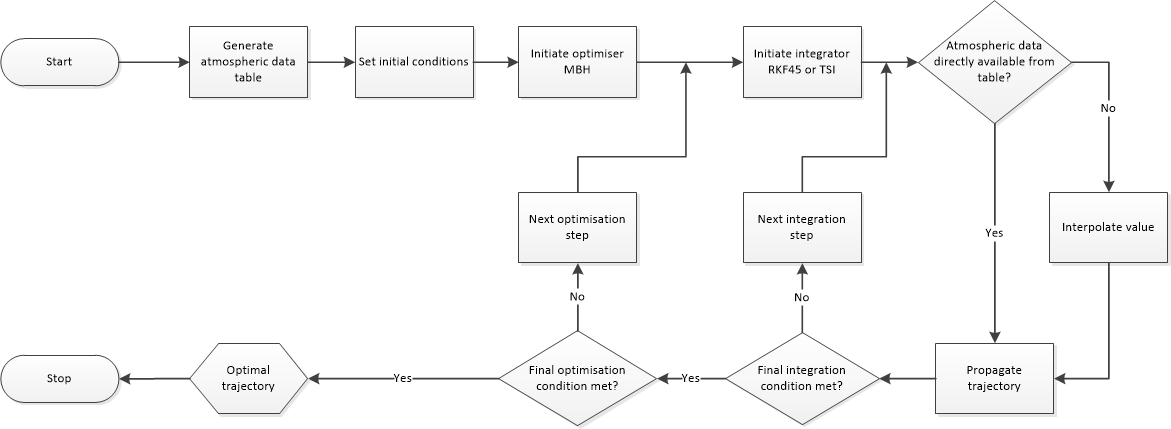
\includegraphics[width=1.0\textwidth]{figures/software/general_soft_architecture.png}
\caption{Proposed general simulation software architecture.}
\label{fig:general_soft_architecture}
\end{figure}

\section{Verification and validation}
\label{sec:vandv}
Each of the written software tools will have to be verified and validated. The verification of a piece of software assures that the software meets the set requirements for the software. If a piece of software is validated, it does what it is suppose to do and the results are correct. For example, it is required of the interpolation tool that it provides a value for $T$, for example, provided a certain $h$ that lies in between the known values. So if the tool is run and it indeed provides a value for $T$ in between the known values, then the tool is verified. However, this does not mean that the value for $T$ is (or comes close to) the correct value (missing minus sign for instance). Therefore, the results have to be compared to a source from which it is known that the values are correct. If the same values are obtained, the tool is validated. Also, each time software is added to the program, the whole program has to be verified and validated again. In this case the interpolation, trajectory propagation, integrators and optimiser all have to be verified and validated. This can consist of different steps. Each of these steps is provided for each of the software tools:

\begin{itemize}
\item \textbf{Interpolation} \textit{Verification:} when the interpolation tool provides a previously unknown value in between two known values after it is run, then it is verified (inspection). \textit{Validation:} two different tables can be generated using Mars-\ac{GRAM} 2005, each with slightly different data points. The interpolation tool will then use the data points of the first table to determine the parameter values of the unknown values corresponding to the $h$, for instance, of the data points of the second table. If the results correspond to the parameter values provided in the second table, the interpolation tool is validated (testing). This can be done for different data point resolutions to determine the minimum resolution required for the table.
\item \textbf{Integrator} \textit{Verification:} to test the integrator by itself, a simple function (with a known outcome) is required. If the integration tool produces results it is verified (inspection). \textit{Validation:} if the results match the known function values then the integrator is also validated. This can be done for increasingly more difficult functions and problems. Examples of validation functions are provided in \cite{noomen2013int} (testing).
\item \textbf{Trajectory propagation} \textit{Verification:} once the integrators have been validated, the trajectory propagation can be incorporated, and it can be checked if it produces proper results (instpection). \textit{Validation:} initially, Apollo ascent flight data \cite{apollo1971} can be used to validate the program for non-atmospheric and Lunar conditions (testing). Then the program shall be validated for Mars ascent using data provided by Woolley \cite{woolley2011mars} for the corresponding conditions (testing). A second Mars validation can be performed by setting specific conditions and simulate the trajectory using other \ac{JPL} software. These results can then be used to validate the thesis software (testing). 
\item \textbf{Optimiser} \textit{Verification:} for an optimiser it is important that it produces a result within a reasonable time. Therefore if the optimiser converges it is verified (inspection). This will initially be done for a benchmark function as provided by \cite{noomen2013}. Once integrated into the simulation program it itself will have to be verified. Again, the desired outcome is a convergence within a reasonable time.  \textit{Validation:} for the initial validation the results will have to match the results of the known function as provided by \cite{noomen2013} (testing). Then the final validation of the complete program will be achieved by creating the same results as presented in \cite{woolley2011mars}, but this time the optimal condition will not be set. Instead the simulation program will have to determine its own optimum conditions, which will then have to correspond to the optimum trajectory results provided in \cite{woolley2011mars}. A further validation of the entire system will then take place using \ac{JPL} optimisation software. In this case an initial condition is set in both the thesis software and the \ac{JPL} software and the optimum result of both programs will be compared to determine the validity of the results obtained (testing).
\end{itemize}

For each piece of software, a walk-through will be performed to verify that each part of the tool is working properly before attempting the final verification. Also, additional validation of the software can be performed using the reference research discussed in \Cref{ch:missher}.


% \Cref{subsec:new_soft} will describe the different elements of the simulation program that will have to be developed and \Cref{subsec:soft_archi} will visualize the top-level architecture of the program as currently envisioned.


%\subsection{New software}
%\label{subsec:new_soft}




%\subsection{Software architecture}
%\label{subsec:soft_archi}

















